
 In figure \ref{2afiveeval} a prediction of $Y(\theta)$, conditional on the 5 evaluated points given in the project descript, as well as a $90\%$ prediction interval is shown.
 
\begin{figure}
    \centering
    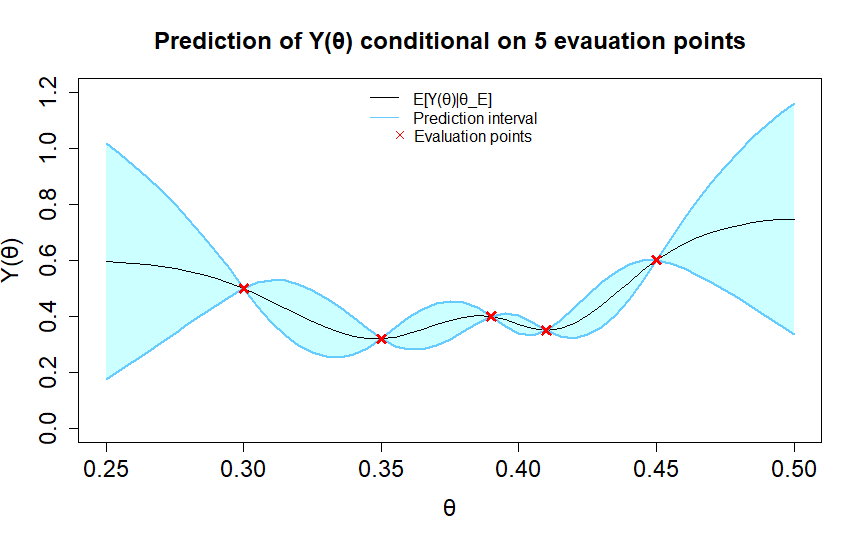
\includegraphics[width=100mm]{2aPlot.png}
    \caption{Prediction of $Y(\theta)$ conditional on the five evaluation points  ($\theta$, $y(\theta)$): $(0.30,0.5)$, $(0.35,0.32)$, $(0.39,0.40)$, $(0.41,0.35)$, and $(0.45,0.60)$. The graph includes a $90\%$ prediction interval. }
    \label{2afiveeval}
\end{figure}


